
\section{Elixir basic typing}

\begin{frame}
\frametitle{Outline} 
\tableofcontents[currentsection]
\end{frame}

\begin{frame}
\frametitle{Putting the theory to work: Elixir}\vspace{-3mm}
\begin{block}{The language}
\begin{itemize}
\item Dynamic and functional, Ruby-like syntax, strong emphasis on metaprogramming
\item Runs on the Erlang VM: distributed and fault-tolerant applications
\item Rich ecosystem of libraries and frameworks, nearly 100K developers
\item In production at Apple, Discord, PepsiCo, BBC, Adobe, Spotify, \ldots
\end{itemize}
\end{block}

\begin{block}{The type system}
\begin{itemize}
\item Since 2021, in collaboration with José Valim (creator of Elixir) and the Dashbit team
\item Based on our set-theoretic types: in the compiler since v1.17 (June 2024),\\
      covers the whole language since v1.20 (current version: 1.20.4, August 2026)
\end{itemize}
\end{block}
\end{frame}


\subsection{Simple function types}


\begin{frame}[fragile]
\frametitle{Static Typing 101}
\begin{block}{A function that always errors}
\begin{minted}[escapeinside=!!]{elixir}
def negate(x) when is_integer(x), do: not x
\end{minted}
\end{block}\pause
\begin{block}{Type error message}
\begin{minted}[escapeinside=!!]{elixir}
Type error:
  |  def negate(x) when is_integer(x), do: not x
                                           ^^^^^
        the operator not expects boolean() as arguments,
        but the argument is integer()
\end{minted}
\end{block}
\end{frame}



% \defverbatim[colored]{\intToInt}{
% \begin{minted}{elixir}
% !\spec! !\po!integer() !\arr! integer()!\pc!
% \end{minted}
% }
\defverbatim[colored]{\intToInt}{
\begin{coloredverbatim}
$ (integer() -> integer())
\end{coloredverbatim}
}
\defverbatim[colored]{\negateInt}{
\begin{minted}{elixir}
def negate(x) when is_integer(x), do: -x
\end{minted}
}

\begin{frame}[fragile]
\frametitle{Types as contracts between functions.}
\pause
\begin{block}{Function A: Negate}
\visible<3->{%
\intToInt
}
\vspace{-2mm}
\visible<2->{%
\negateInt
}
\vspace{-1.8mm}
\end{block}
\pause\pause
\begin{block}{Function B: Subtract}
\vspace{-1mm}
\begin{coloredverbatim}
$ (integer(), integer() -> integer())
\end{coloredverbatim}
\vspace{-2mm}
\begin{minted}[escapeinside=!!]{elixir}
def subtract(a, b) when is_integer(a) and is_integer(b) do
    a + negate(b)
end
\end{minted}
\end{block}
\pause
\begin{block}{Question}
\begin{itemize}
    \item What if we modify the implementation of \code{negate}?
\end{itemize}
\end{block}
% \begin{block}{Answer}
% If the implementation of \code{negate} changes and violates the type contract, it could lead to unexpected behavior or errors in the \code{subtract} function. Ensuring that the contract is maintained helps guarantee the correctness of our code.
% \end{block}
\end{frame}

\defverbatim[colored]{\intBool}{
\begin{coloredverbatim}
$ (integer() \oor boolean()) -> (integer() \oor boolean())
\end{coloredverbatim}
}
\defverbatim[colored]{\negateBool}{
\begin{minted}{elixir}
def negate(x) when is_boolean(x), do: not x
\end{minted}
}



\subsection{Unions, intersections, negations}

\begin{frame}[fragile]{Union types: correct, but not precise enough.}
\vspace{-2mm}
\begin{block}{Adding a clause for booleans}
\visible<2->{%
\intBool
}
\vspace{-2.1mm}
\visible<1->{%
\negateInt
\vspace{-2.1mm}
\negateBool
}
\vspace{-2.2mm}
\end{block}
\pause\pause

\vspace{-4mm}

\begin{block}{\vspace{-5mm}}
\vspace{-0.2mm}
\begin{coloredverbatim}
$ (integer(), integer() -> integer())
\end{coloredverbatim}
\vspace{-2.1mm}
\begin{minted}[escapeinside=!!]{elixir}
def subtract(a, b) when is_integer(a) and is_integer(b) do
    a + negate(b)
end
\end{minted}
\end{block}
\pause
\begin{block}{Type error in subtract}
\begin{minted}[fontsize=\footnotesize]{elixir}
Type error:
  | def subtract(a, b) when is_integer(a) and is_integer(b) do
  |   a + negate(b)
        ^ the operator + expects integer(), integer() as arguments,
          but the second argument can be integer() or boolean()
\end{minted}
\end{block}
\end{frame}
% todo: add notes with pdfpc
% \begin{block}{Explanation}
% The `+` operator expects two integer arguments, but the second argument can now be an integer \emph{or} a boolean due to the changes in the `negate` function. 
% \end{block}
\defverbatim[colored]{\intersection}{
\begin{coloredverbatim}
$ (integer()->integer()) \oand (boolean()->boolean())
\end{coloredverbatim}
}
\defverbatim[colored]{\intersectionHalf}{
\begin{coloredverbatim}
$ (integer()->integer()) \oand
\end{coloredverbatim}
}
\defverbatim[colored]{\negateIntBool}{
\begin{minted}[escapeinside=!!]{elixir}
def negate(x) when is_integer(x), do: -x
def negate(x) when is_boolean(x), do: not x
\end{minted}
}

\defverbatim[colored]{\intersection}{
\begin{coloredverbatim}
$ (integer()->integer()) \oand (boolean()->boolean())
\end{coloredverbatim}
}
\defverbatim[colored]{\intersectionHalf}{
\begin{coloredverbatim}
$ (integer()->integer()) \oand
\end{coloredverbatim}
}
\defverbatim[colored]{\negateIntBool}{
\begin{minted}[escapeinside=!!]{elixir}
def negate(x) when is_integer(x), do: -x
def negate(x) when is_boolean(x), do: not x
\end{minted}
}


\begin{frame}[fragile]
\frametitle{Type intersections for functions.}
\begin{block}{A more precise annotation}
\vspace{-4.9mm}
\begin{overlayarea}{\textwidth}{.8cm}
% \only<2>{\intersectionHalf}
\only<2->{\intersection}    
\end{overlayarea}
\vspace{.4mm}
% \hfill
% \vspace{1mm}
\negateIntBool
\vspace{-0.7mm}
\end{block}
\pause\pause
\begin{block}{The function \texttt{subtract} type checks}
\vspace{-2mm}
\begin{coloredverbatim}
$ (integer(), integer() -> integer())
\end{coloredverbatim}
\vspace{-2.1mm}
\begin{minted}[escapeinside=!!]{elixir}
def subtract(a, b) when is_integer(a) and is_integer(b) do
    a + negate(b)
end
\end{minted}
\end{block}
\end{frame}

\defverbatim[colored]{\lognegType}{
\begin{coloredverbatim}
$ (false \oor nil -> true) \oand (\onot (false \oor nil) -> false)
\end{coloredverbatim}
}
\defverbatim[colored]{\lognegSingle}{
\begin{coloredverbatim}
$ (false \oor nil -> true) \oand
\end{coloredverbatim}
}

\begin{frame}[fragile]
\frametitle{Singleton and Negation Types}
\begin{block}{Logical negation}%
\vspace{-9mm}
\begin{overlayarea}{\textwidth}{0.5mm}%
    \only<2>{\lognegSingle}
\only<3>{\lognegType}
\end{overlayarea}%
\hfill \vspace{1mm}
\begin{minted}[escapeinside=||]{elixir}
def logical_neg(x) when x == false or x == nil, do: true
def logical_neg(x), do: false
\end{minted}
\end{block}
\pause
\begin{block}{Types}
\begin{itemize}
    \item Singleton types are types containing exactly one value
    \visible<3->{\item Negation types contain any value that is \emph{not} in the 
    negated type.}
\end{itemize}
\end{block}

\end{frame}

\defverbatim[colored]{\mapSip}{
\begin{coloredverbatim}
$ ([a], (a -> b)) -> [b] \owhen a: term(), b: term()
\end{coloredverbatim}
}
\defverbatim[colored]{\mapSigMinted}{
\begin{minted}{elixir}
!\spec! ([a], (a -> b)) -> [b] !\when! a: term(), b: term()
\end{minted}
}
\defverbatim[colored]{\map}{
\begin{minted}[escapeinside=!!]{elixir}
def map([h | t], fun), do: [fun.(h) | map(t, fun)]
def map([], _fun), do: []
\end{minted}
}


\subsection{Polymorphism}
\begin{frame}[fragile]
\frametitle{Polymorphism with Local Type Inference}

\begin{block}{Expressions and functions can have types containing type variables}
\vspace{-7.2mm}
\begin{overlayarea}{\textwidth}{2mm}
\only<2->{\mapSip}
% \only<2->{\mapSigMinted} 
\end{overlayarea} 
\hfill \vspace{1.4mm}
\visible<1->{\map}
\vspace{-1.5mm}
\end{block}
\pause
\begin{block}{Type Variables}
    \begin{itemize}
        \item Quantified using a postfix \texttt{\color{typeBrique}when} with upper bounds
        % \item First-order polymorphism only
    \end{itemize}
\end{block}
\pause
\begin{block}{System deduces type variable instantiation}
\begin{minted}{elixir}
map([{0, true}], fn {x, y} when is_integer(x) -> x end)
# type [integer()]
\end{minted}
\end{block}
\end{frame}

\defverbatim[colored]{\logorFinal}{
\begin{coloredverbatim}
$ ((false \oor nil, a) -> a) when a: term()
$ (a, term() -> a) when a: \onot(false or nil)
\end{coloredverbatim}
}
\defverbatim[colored]{\logorFirst}{
\begin{coloredverbatim}
$ ((false \oor nil, a) -> a) \oand 

\end{coloredverbatim}
}
\defverbatim[colored]{\logorSecond}{
\begin{coloredverbatim}
$ ((false \oor nil, a) -> a) \oand 
  ((b, term()) -> b) \owhen a: term(), b: \onot(false \oor nil)
\end{coloredverbatim}
}


\begin{frame}[fragile]{Intersection and polymorphism}\transdissolve<4->

\begin{block}{Logical OR}%
\vspace{-7mm}
\begin{overlayarea}{\textwidth}{2mm}
    \only<2>{\logorFirst}
    \only<3->{\logorSecond}
    % \only<4>{\logorFinal}
\end{overlayarea}%
\hfill \break 
\begin{minted}[escapeinside=!!]{elixir}
def logical_or(x, y) when x == false or x == nil, do: y
def logical_or(x, _), do: x
\end{minted}
\end{block}
\pause\pause\pause\pause
\textbf{\color{darkslateblue}Bounded Polymorphism:}
\[\color{typeBrique}\forall (s{\leq}\alpha{\leq} u).t \quad\stackrel{def}{=}\quad (\forall \alpha).t[\alpha:=(s{\vee}(\alpha{\wedge} u))]\]
\only<4>{\begin{textblock}{5}(0,0)
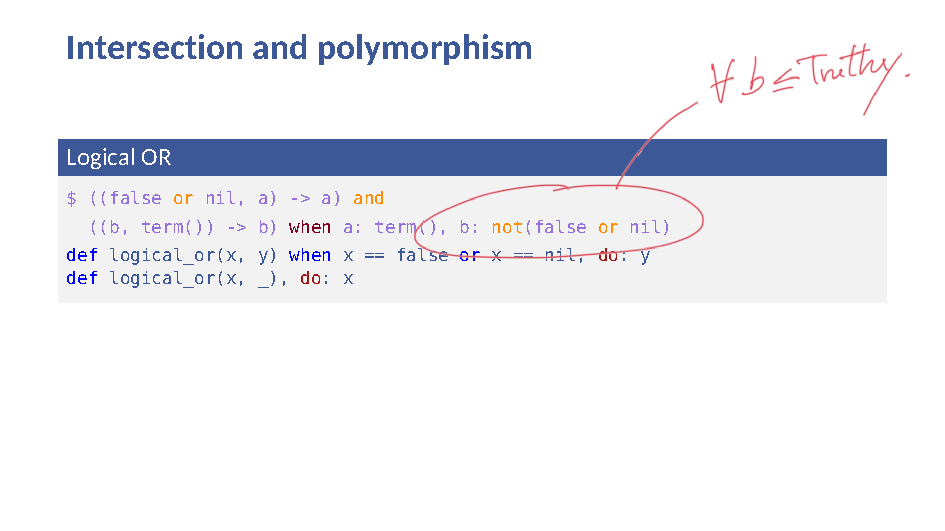
\includegraphics[scale=1]{images/slide-bounded_q.pdf}
\end{textblock}}
\end{frame}





\section{Guard analysis}
\begin{frame}
\frametitle{Outline} 
\tableofcontents[currentsection]
\end{frame}


\subsection{Case expressions: redundancy, exhaustiveness, and narrowing}

\begin{frame}[fragile]
\frametitle{Pattern Matching: Case expressions}
\begin{block}{Using a case expression}
\begin{minted}[escapeinside=!!]{elixir}
def negate(x), do: (case x do
  x when is_integer(x) -> -x
  x when is_boolean(x) -> not x
end)
\end{minted}
\end{block}

\begin{block}{Using multiple function clauses}
\begin{minted}[escapeinside=!!]{elixir}
def negate(x) when is_integer(x), do: -x
def negate(x) when is_boolean(x), do: not x
\end{minted}
\end{block}

\textbf{\color{darkslateblue}Both are equivalent, but the second is preferred in Elixir.}
\end{frame}

\defverbatim[colored]{\result}{
%\vspace{-1.5mm}
\begin{minted}[escapeinside=||,fontsize=\small]{elixir}
|\spec| |\ty| result() = 
    %{output: :ok, socket: socket()} or
    %{output: :error, message: :timeout or {:delay, integer()}}
\end{minted}
\vspace{-1.5mm}
}

\begin{frame}[fragile]
\frametitle{Exhaustiveness and redundancy checking}
\vspace{-7mm}
\begin{block}{\vspace{-5mm}}
\result
\end{block}
\pause

\begin{block}{Exhaustiveness checking: handling all cases}
\begin{minted}[escapeinside=||,fontsize=\small]{elixir}
|\spec| result() -> string()
def handle(r) when r.output == :ok, do: "Msg received"
def handle(r) when r.message == :timeout, do: "Timeout"
\end{minted}
\pause
\vspace{-1.8mm}
\begin{minted}[fontsize=\small]{elixir}
#=> Type Warning: non-exhaustive pattern matching
\end{minted}
\end{block}
\pause

\defverbatim[colored]{\unusedBranch}{
\begin{minted}[fontsize=\small]{elixir}
#=> Type Warning: unused branch
\end{minted}
}

\begin{block}{Redundancy checking: detecting unused clauses}
\begin{minted}[escapeinside=||,fontsize=\small]{elixir}
|\spec| result() -> string()
def handle(r) when r.output == :ok, do: "Msg received"
def handle(r) when r.output == :error, do: "Error raised"
def handle(%{socket: _}), do: "Socket found"
\end{minted}
\pause%
\vspace{-1.6mm}\unusedBranch\vspace{-1.7mm}
\end{block}
\end{frame}

% add a fourth branch for overlapping, by matching 
% on :socket

% remove? no time
\begin{frame}[fragile]
\transdissolve
\frametitle{Narrowing: inferring more precise types}

\vspace{-11mm}%was \vspace{-4mm}
\begin{block}{\vspace{-5mm}}
\result
\end{block}\pause
\begin{block}{Automatically infer a return type}
\begin{minted}[escapeinside=||,fontsize=\footnotesize]{elixir}
|\spec| result() -> _
def handle(r) when r.output == :ok, do: {:accepted, r.socket}
def handle(r) when is_atom(r.message), do: r.message
def handle(r), do: {:retry, elem(r.message, 1)}
\end{minted}
\pause\vspace{-1.7mm}
\begin{minted}[fontsize=\footnotesize]{elixir}
#=> Return type: {:accept, socket()} or :timeout or {:retry, integer()}
\end{minted}
\vspace{-1.2mm}
\end{block}
\pause\pause\pause\pause
\begin{block}{Inferring a more precise type}
\begin{minted}[fontsize=\footnotesize,escapeinside=||]{elixir}
|\spec| (%{output: :ok, socket: socket()} -> {:accept,socket()}) and
  (%{output: :error, message: :timeout} -> :timeout) and
  (%{output: :error, message: {:delay,integer()}} -> {:retry,integer()})
\end{minted}
\end{block}
\only<4>{\begin{textblock}{5}(0,0)
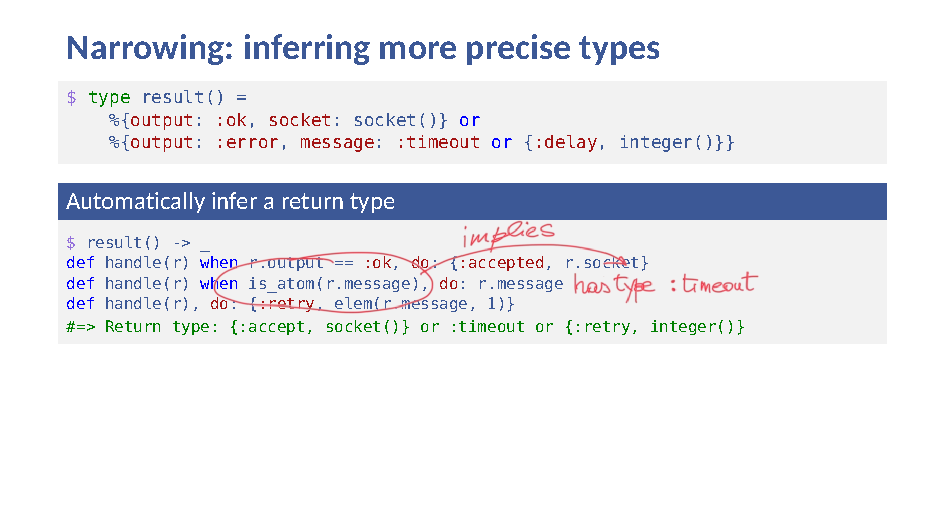
\includegraphics[scale=1]{images/slide-narrow1.pdf}
\end{textblock}}

\only<5>{\begin{textblock}{5}(0,0)
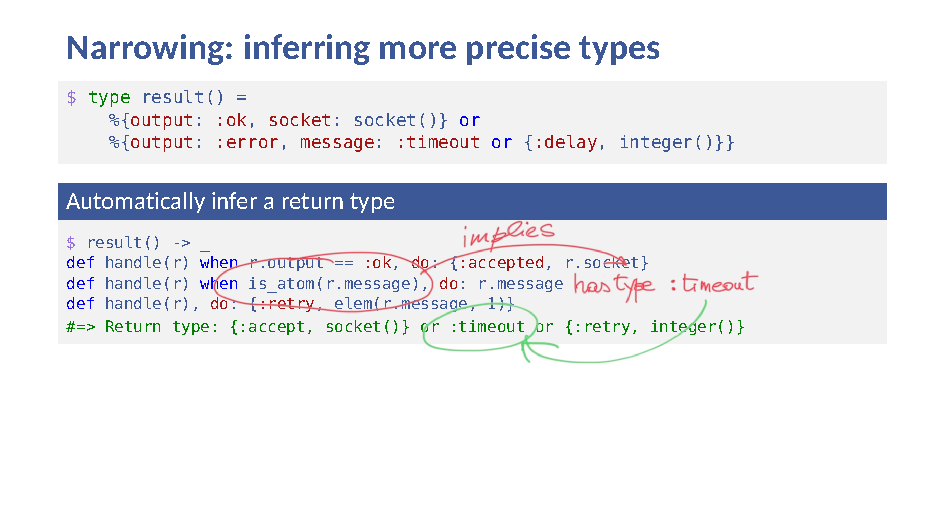
\includegraphics[scale=1]{images/slide-narrow2.pdf}
\end{textblock}}
\only<6>{\begin{textblock}{5}(0,0)
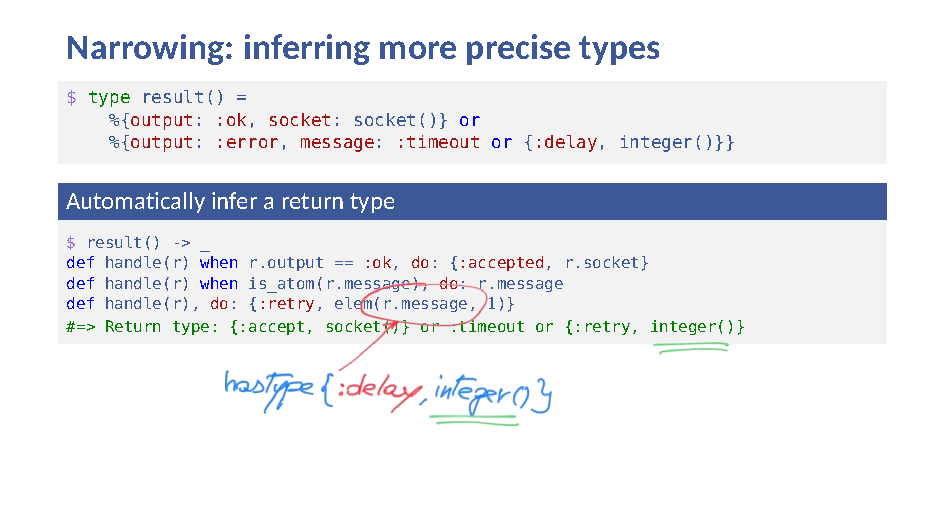
\includegraphics[scale=1]{images/slide-narrow3.pdf}
\end{textblock}}

\only<8>{\begin{textblock}{5}(0,0)
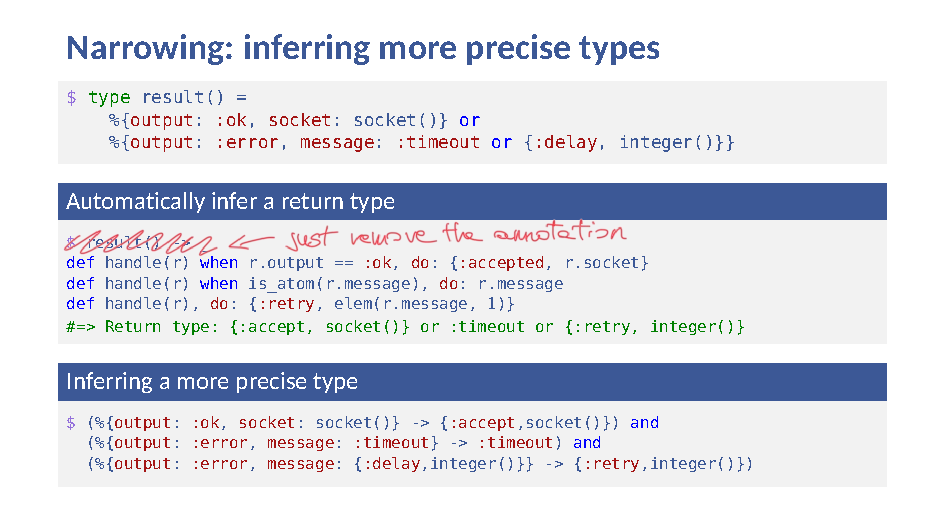
\includegraphics[scale=1]{images/slideNarrowing.pdf}
\end{textblock}}
\end{frame}

